
\subsection{Definition}

\textbf{Dynamic programming} is a method by recurrence in order to solve complex problem.
\begin{itemize}
    \item breaking it down into a collection of simpler subproblems
    \item solving each of those subproblems just once, and storing their solutions in memory
    \item[$\rightarrow$] Next time the same subproblem occurs, instead of 
recomputing its solution, only looks up to the previously computed solution.
Thereby \textbf{saving computation time at the expense of storage space}.
\end{itemize}

\subsection{Solving the knapsack problem with DP}

\subsubsection{The knapsack problem}
\begin{itemize}
    \item A set of item $I$
    \item for each item $i \in I$ is associated a value $v_i$ and a weight $w_i$.

    \item[Goals] 
        \begin{tabular}{m{3cm}m{12cm}}
            $\sum_{i \in I} v_i x_i$: & Maximize the value of selected items\\
            $\sum_{i \in I} w_i x_i \le C$ & Under constraint that the total
            capacity cannot exceed a given maximal capacity $C$ \\ 
            $x_i \in \{0,1\}$ & And an item cannot be partially selected \\
        \end{tabular}
\end{itemize}

Note that Knapsack is an NP-Complete problem as it can be used
to find a solution to the subset-sum problem, which is NP-complete.

\paragraph{Subset-sum problem}

Given a set of natural number and a capacity K. 
Find a subset S such that :
$$\sum_{i \in S} c_i = K$$


\subsubsection{Solutions}
\begin{itemize}
    \item \textbf{DP for knapsack in 0(Cn)}.

        Refer to the optimal objective of the problem with capacity $k$ and
        items \{1,…,j\} $\in$ I as $O(k,j)$. We can easily notice that :

        \begin{itemize}
            \item $O(k,0) = 0 \text{\footnotemark}$
            \item $ O(k,j) = \begin{cases} 
                    max(O(k,j-1) , vj +O(k-wj,j-1))\text{\footnotemark} & if \quad w_j \leq k \\
                    O(k,j-1) & otherwise
                \end{cases}$
        \end{itemize}
        \footnotetext{As their are no elements to choose from}
        \footnotetext{Bellman's equations}


        \begin{lstlisting}[caption=Knapsack DP]
val items = Array((1,1),(6,2),(18,5),(22,6),(28,7)) // (value,weight)
val C = 11
def O(j: Int, k: Int): Int = {
    if (j < 0) 0
    else {
        val (vj,wj) = items(j)
        if (wj > k) O(j-1,k)
        else O(j-1,k).max(vj + O(j-1,k-wj))
    }
}
println(O(items.size-1,C))
        \end{lstlisting}

        \begin{center}
    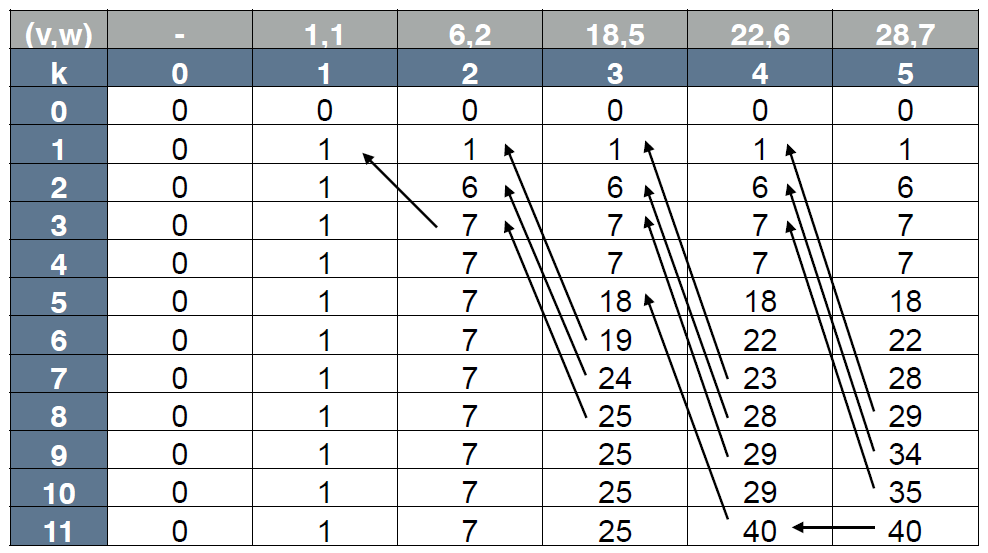
\includegraphics[width=7cm]{KnapsackDP.png}
        \end{center}

    \item \textbf{DP for knapsack in 0(Vn)}.

        Using a similar logic, it is also possible to define an algorithm which
        run in $\theta$(Vn) to compute knapsacks. Let $V = \sum_{i \in I} v_i$,
        we can redefine O(k,j) as O(w,j), the optimal weight using only items
        \{1,...,j\}. The equation will thus change as follow :

    \begin{itemize}
    \item $O(0,j) = O(p,0) = 0 \text{\footnotemark} $
    \item $ O(p,j) = \begin{cases}
                min(O(p,j-1), wi + O(p-v_j,j-1)) & if \quad v_j \leq p \\
                O(p,j-1) & otherwise
            \end{cases}$
        \end{itemize}
        \footnotetext{As $w_i > 0$ for all $i \in I$ and as we cannot have w > 0 with 
        an empty set.}
        \begin{center}
            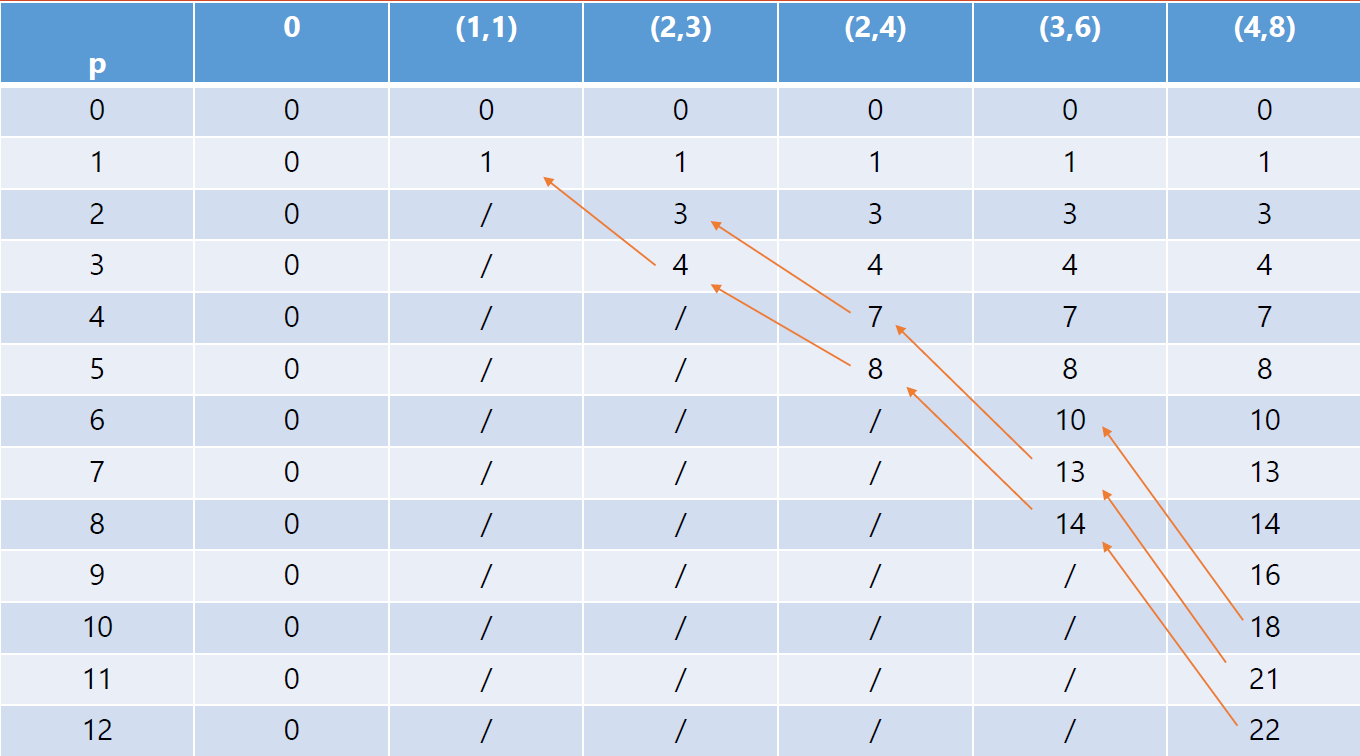
\includegraphics[width=7cm]{KnapsackDPAlgo2.png}
        \end{center}
\end{itemize}

\subsubsection{Cache usage}
\begin{tabular}{m{9cm}m{6cm}}
As explain, a cache is use in order to store computed value and avoid to recompute
it. In \textcolor{red}{red} we have the cells actually computed.
&
    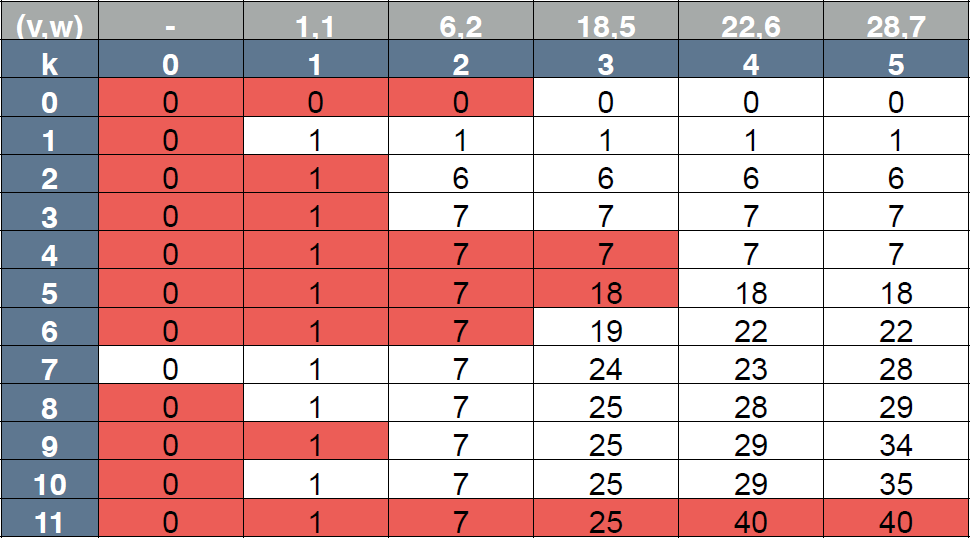
\includegraphics[width=6cm]{KnapsackDPAlgo1.png}
\end{tabular}


\subsubsection{Pseudo-polynomial}

DP is \textsc{pseudo-polynomial}, since it is exponential in the 
\textit{length of input} ($log(C)$) which is the number of bits required to
encode the input ($C$). The complexity is thus exponential relatively to the
input size. This algorithm is \textbf{weakly NP-Complete} or
\textbf{pseudo-polynomial}\footnote{a numeric algorithm runs in
pseudo-polynomial time if its running time is polynomial in the numeric value
of the input, but is exponential in the length of the input – the number of
bits required to represent it.} as it is roughly polynomial for small values of
C while computing larger value is much more expensive\footnote{Not all
    NP-Complete algorithm are pseudo polynomial ! Like the traveling salesman
problem (TSP), for example.}.


\subsection{Other examples of DP algorithms}

Before reading this section, please remember that all algorithm that can be
implemented via dynamic programming are not ipso-facto pseudo polynomial ! Any
algorithm can be expressed with dynamic programming as long as it can be separated in
sub problems.

%\subsubsection{TSP}
%Say $1$ be the source of the TSP.
%\begin{itemize}
%    \item $O(S,1) = 0 $
%    \item $ O(S, j) = 
%        min\Bigg( \{ \quad O\bigg(S -\{j\}, i\bigg) + d_{ij} \quad
%            |\quad  i \in S \wedge i \in
%        Neighboor(j)\quad \} \Bigg)$
%\end{itemize}
%
%The answer to join $1$ to $n$ is $O(AllVertex, n)$


\subsection{Exam}
I give you a problem (for instance the TSP, Knapsack)
\begin{itemize}
    \item  Design a greedy algorithm
    \item  Design a Dynamic Programming formulation
    \item  Design a relaxation and upper/lower bound
        procedure and embed it in a Branch and Bound
    \item  Justify advantages and disadvantages of each
    \item  Apply the three techniques to a small instance
        manually
\end{itemize}
